\chapter*{BDD from 5,000 feet}

\ifnotes

    \section*{Learning Outcomes}
    
    \begin{itemize}
        \item Arrange the BDD practices correctly
        \item Explain that Exploratory Testing requires test skills
        \item Explain that test automation requires dev skills
        \item Describe who gets involved in each step
        \item Describe how these steps fit into a typical agile process
    \end{itemize}

    \section*{Setup}
    
    This is as important as Example Mapping. Positioned at the end of the day, this exercise is where we bring it all together.
    
    Before starting, explain that the colour coding is significant and that some arrows have been omitted to keep the diagram readable. Give them ten minutes or so to arrange the steps.
    
    \section*{Review}
    
    First, go through the nodes. This order works well:
    
    \begin{itemize}
        \item Nodes 5, 6, 7 - ask "did you spot the Red/Green/Refactor TDD loop?". This gets them started, then work back from there. 
        \item Node 4 is where a scenario gets automated. This requires someone with dev skills.
        \item Node 3 is where the living documentation is created.
        \item Node 2 is where Example Mapping happens
        \item Node 1 is where requirement elicitation and story prioritisation happens
        \item Node 8 you may have to give a brief explanation of exploratory testing, an contrast it from formal test plans as well as a PO just trying a few things. Ask "what happens if an exploratory test fails?" - "it depends" - draw red arrows to nodes 1, 2, 3, 4, 5. Also there's a missing green arrow from 8 to 1, because we don't always release.
        \item Node 9 mention Continuous Delivery/Deployment if appropriate
    \end{itemize}
    
    Then talk about who does what. Start at Node 1:
    
    \begin{itemize}
        \item Node 1 PO/BA/customer        
        \item Node 2 3-Amigos. At least one representative from business, dev, test. Keep the meeting 6 or fewer people. 
        \item Node 3 Ideally 3 Amigos. Next best is Dev/Test with mandatory PO/BA review -because this gives feedback that the knowledge has been successfully transmitted to the dev/test folk. Some orgs have PO/BA write the GWT, but this obscures knowledge transfer and dev/test often change the GWT to make automation easier.
        \item Node 4 Needs dev skills. Mature teams sometimes have reusable libraries that make this automation simpler.
        \item Nodes 5, 6, 7 - Devs. Good place to pair with testers fo cross/up-skilling        
        \item Node 8 Needs test skills
        \item Node 9 Depends
    \end{itemize}
    
    The ask when should these activities take place (n-1=iteration before story is scheduled, n=iteration in which story is being implemented, n+1=iteration after story has been delivered):
    
     \begin{itemize}
        \item Node 1 n-1 (or earlier)        
        \item Node 2 n-1. Business to publicise story(s) at least the day before. Timebox for 30 minutes. Hold regularly - schedule every day if possible. Leads to shorter grooming/estimating/planning meetings
        \item Node 3 Preferably n-1, sometimes n
        \item Node 4 Either n-1 or n 
        \item Nodes 5, 6, 7 Always n        
        \item Node 8 Either n or n+1 (or later)
        \item Node 9 Either n or n+1 (or later)
    \end{itemize}
   
    
    Remind them that the answer, and a spare diagram, is on the last page of the workbook.
\fi 

\ifcontent

    Let's look at an overview of the BDD process, and how it fits into your existing agile process activities.
    
    \section*{Arrange the steps}
    
    Consider the process steps below. Some of these are steps your team may already be doing, and some may be unfamiliar to you.
    
    The flow diagram below represents the key parts of a typical BDD workflow.
    
    Work in pairs to arrange the steps into order in the diagram. If you're not sure, just take a guess. Don't feel bad if you don't know!
    
    \NOTSTANDARD{
        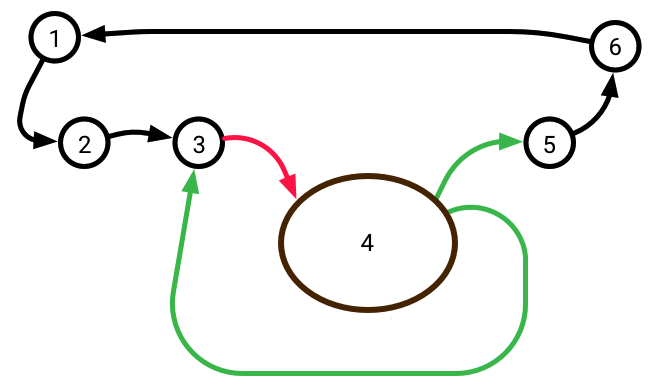
\includegraphics[width=\textwidth]{images/bdd-process-without-TDD}
    
        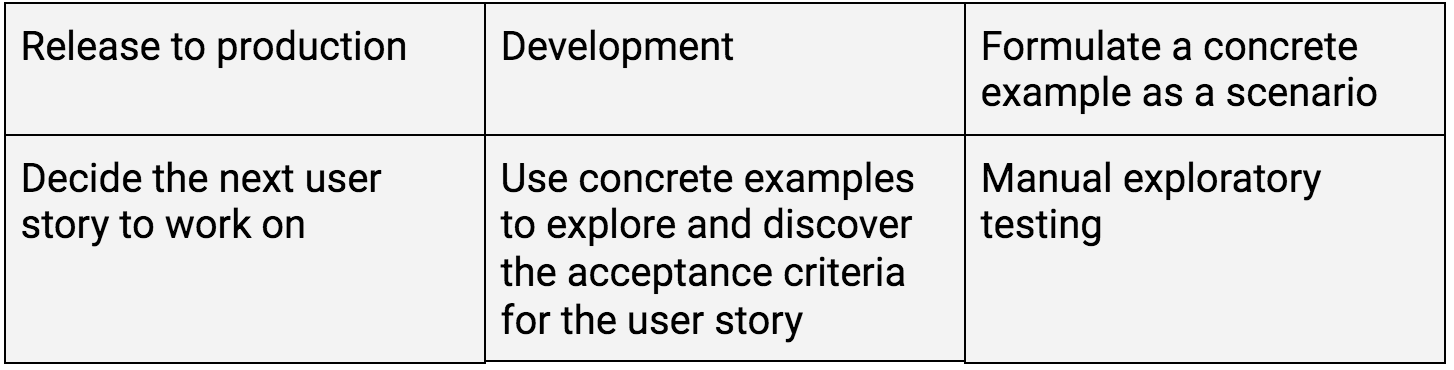
\includegraphics[width=\textwidth]{images/bdd-process-table-without-TDD}
    }
    \STANDARD{
        \begin{center}
            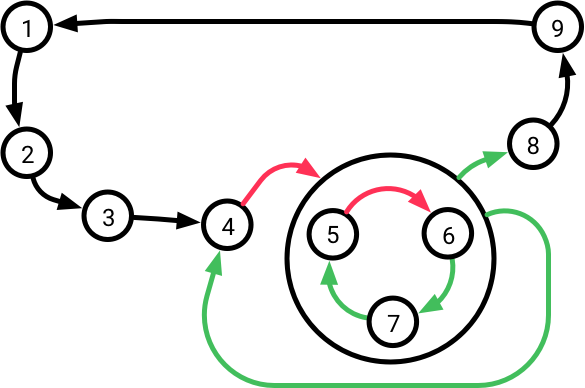
\includegraphics[height=9cm]{images/bdd-process}
            
            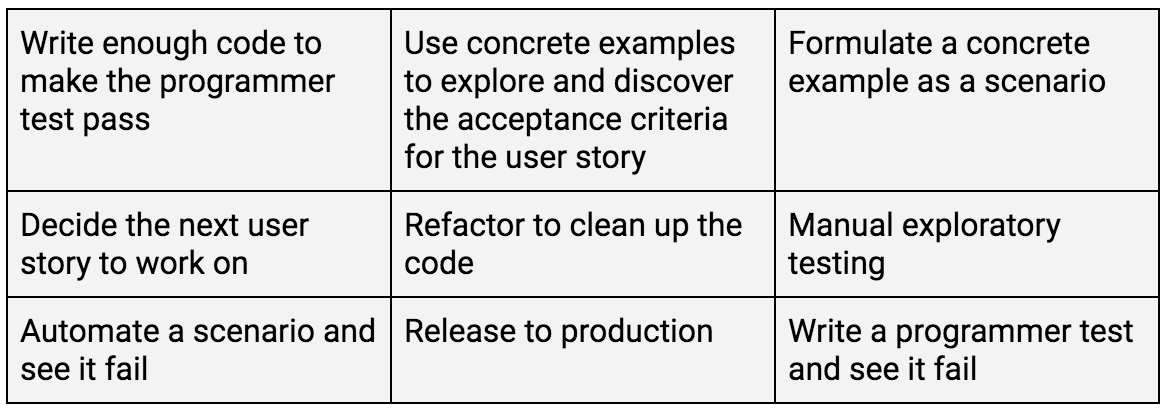
\includegraphics[width=\textwidth]{images/bdd-process-table}
        \end{center}
    }

\fi
